% !TEX root = ../main.tex

% 中英标题：\chapter{中文标题}[英文标题]
\chapter{噪声感知与偏好提取的多行为推荐方法}

\section{引言}
随着互联网平台中用户行为的多样化，\textbf{多行为推荐系统}逐渐成为解决推荐系统中\textbf{数据稀疏}和\textbf{冷启动}问题的有效工具。传统的推荐算法通常依赖单一类型的用户行为（如购买行为）来推测用户的偏好，这种方法在面对数据稀疏或冷启动时会遇到显著挑战。为了解决这些问题，多行为推荐系统通过引入辅助行为（例如点击、浏览、收藏等）来增强对用户兴趣的理解，从而提高推荐精度。然而，在实际应用中，辅助行为往往含有大量噪声信息，例如误点击、无意浏览或无效收藏等，这些噪声交互可能严重干扰对用户真实偏好的识别。

尽管近年来针对多行为推荐的研究不断深入，已有的一些工作主要集中在\textbf{行为信息融合}和\textbf{行为关系建模}上，但大多数方法忽视了辅助行为中的噪声问题。现有的多行为推荐算法通常假设所有辅助行为均为有效信息，未能有效区分低质量的噪声行为与真实的用户兴趣。此外，传统的去噪方法多集中在单一行为场景中，忽略了多行为场景下\textbf{行为间的关联性}，以及如何利用高质量辅助行为增强目标行为的表达能力。

针对上述挑战，本文提出了一种新颖的框架——\textbf{噪声感知与偏好提取的多行为推荐方法（Noise Identification and Preference Extraction in Multi-Behavior Recommender System, NIPER）}。该框架由两个主要模块组成，旨在有效识别并去除辅助行为中的噪声，同时增强辅助行为与目标行为之间的互补信息，提升推荐精度和系统的鲁棒性。

首先，\textbf{跨行为与行为内加权去噪模块}旨在识别不同用户行为对偏好的影响差异，为每种行为分配不同的权重。在此基础上，本文采用跨行为与行为内信息融合的策略，区分噪声交互与有效交互。通过去除低权重的噪声交互，显著提升了对用户真实偏好的学习效果。

其次，\textbf{基于偏好信息的表征增强模块}采用自监督学习策略增强辅助行为与目标行为之间的信息传递。通过生成正负样本对促进目标行为的学习，并匹配用户和物品的相似交互嵌入，进一步增强了行为间的一致性与准确性。该方法不仅缓解了目标行为数据稀疏问题，还揭示了用户在不同交互场景下的潜在兴趣偏好。

本文的主要贡献如下：

\begin{enumerate}
    \item 本文提出了一个能够有效识别多行为推荐系统中噪声并提取真实偏好的框架，为多行为推荐的去噪研究提供了新的视角。
    \item 本文提出了一种新的跨行为与行为内加权去噪模块，通过引入加权机制，有效识别并去除辅助行为中的噪声，提升了模型对真实用户偏好的学习能力。
    \item 本文设计了一种创新的自监督学习方法，利用辅助行为数据中的真实偏好补充目标行为，从而缓解目标行为数据稀疏问题，并揭示用户与物品之间的相似交互模式。
\end{enumerate}

综上所述，本研究不仅提升了多行为推荐系统的准确性和鲁棒性，也为推荐系统中的去噪问题提供了新的思路。实验结果表明，NIPER 在多个公开数据集上显著优于现有的多行为推荐方法，展现出优越的性能与泛化能力。

\section{问题定义及方法概述}

\subsection{问题定义}

在本研究中，定义用户集合为 $ U = \{u_1, u_2, ..., u_{|U|}\} $，物品集合为 $ I = \{i_1, i_2, ..., i_{|I|}\} $，其中 $ |U| $ 和 $ |I| $ 分别表示用户和物品的数量。符号 $ B $ 表示行为类型的集合。  

在数据集中，将购买行为设定为\textbf{目标行为}，而其他行为（如浏览、加购、收藏等）设定为\textbf{辅助行为}，并用 $ K $ 表示行为类别的总数。  

构建的用户–物品交互图记为 $ G^R = (V, E^R) $，其中 $ V = U \cup I $ 表示图中所有用户与物品节点的集合，边集 $ E^R $ 表示观测到的交互关系。在包含 $ K $ 种行为的多行为场景下，整体交互图 $ G^R $ 可划分为 $ K $ 个行为子图：$ G^R_1, G^R_2, ..., G^R_K $。  

给定用户与物品之间的交互矩阵集合 $ R $，其中 $ R_k \in \mathbb{R}^{|U| \times |I|} $ 表示第 $ k $ 种行为下的交互矩阵。若 $ R^k_{ui} = 1 $，则表示用户 $ u $ 在行为 $ k $ 下与物品 $ i $ 发生过交互，此时在行为图 $ G^R_k $ 中存在一条连接用户 $ u $ 与物品 $ i $ 的边；若 $ R^k_{ui} = 0 $，则表示用户 $ u $ 在该行为下未与物品 $ i $ 交互。  

为了进一步挖掘用户与物品之间潜在的相似偏好信息，构建了\textbf{用户同构图} $ G^U $ 和\textbf{物品同构图} $ G^I $，以捕捉用户–用户及物品–物品之间的共享交互关系。在构建过程中，遍历各行为下的用户–物品交互记录；若一对用户 $ (u, v) $ 或一对物品 $ (i, j) $ 在目标行为（购买行为）下存在共同交互，则在图 $ G^U $ 中连接 $ u $ 与 $ v $，并在图 $ G^I $ 中连接 $ i $ 与 $ j $。  

多行为推荐任务的形式化定义如下：  

\begin{itemize}
    \item \textbf{输入}：用户在 $ K $ 种行为下的交互图集合 $ \{G^R_1, G^R_2, ..., G^R_K\} $；
    \item \textbf{输出}：一个推荐模型，用于预测用户 $ u $ 在第 $ K $ 种行为（即目标行为）下与物品 $ i $ 发生交互的概率。
\end{itemize}

\subsection{算法实现概述}

\begin{figure}[h]
\centering
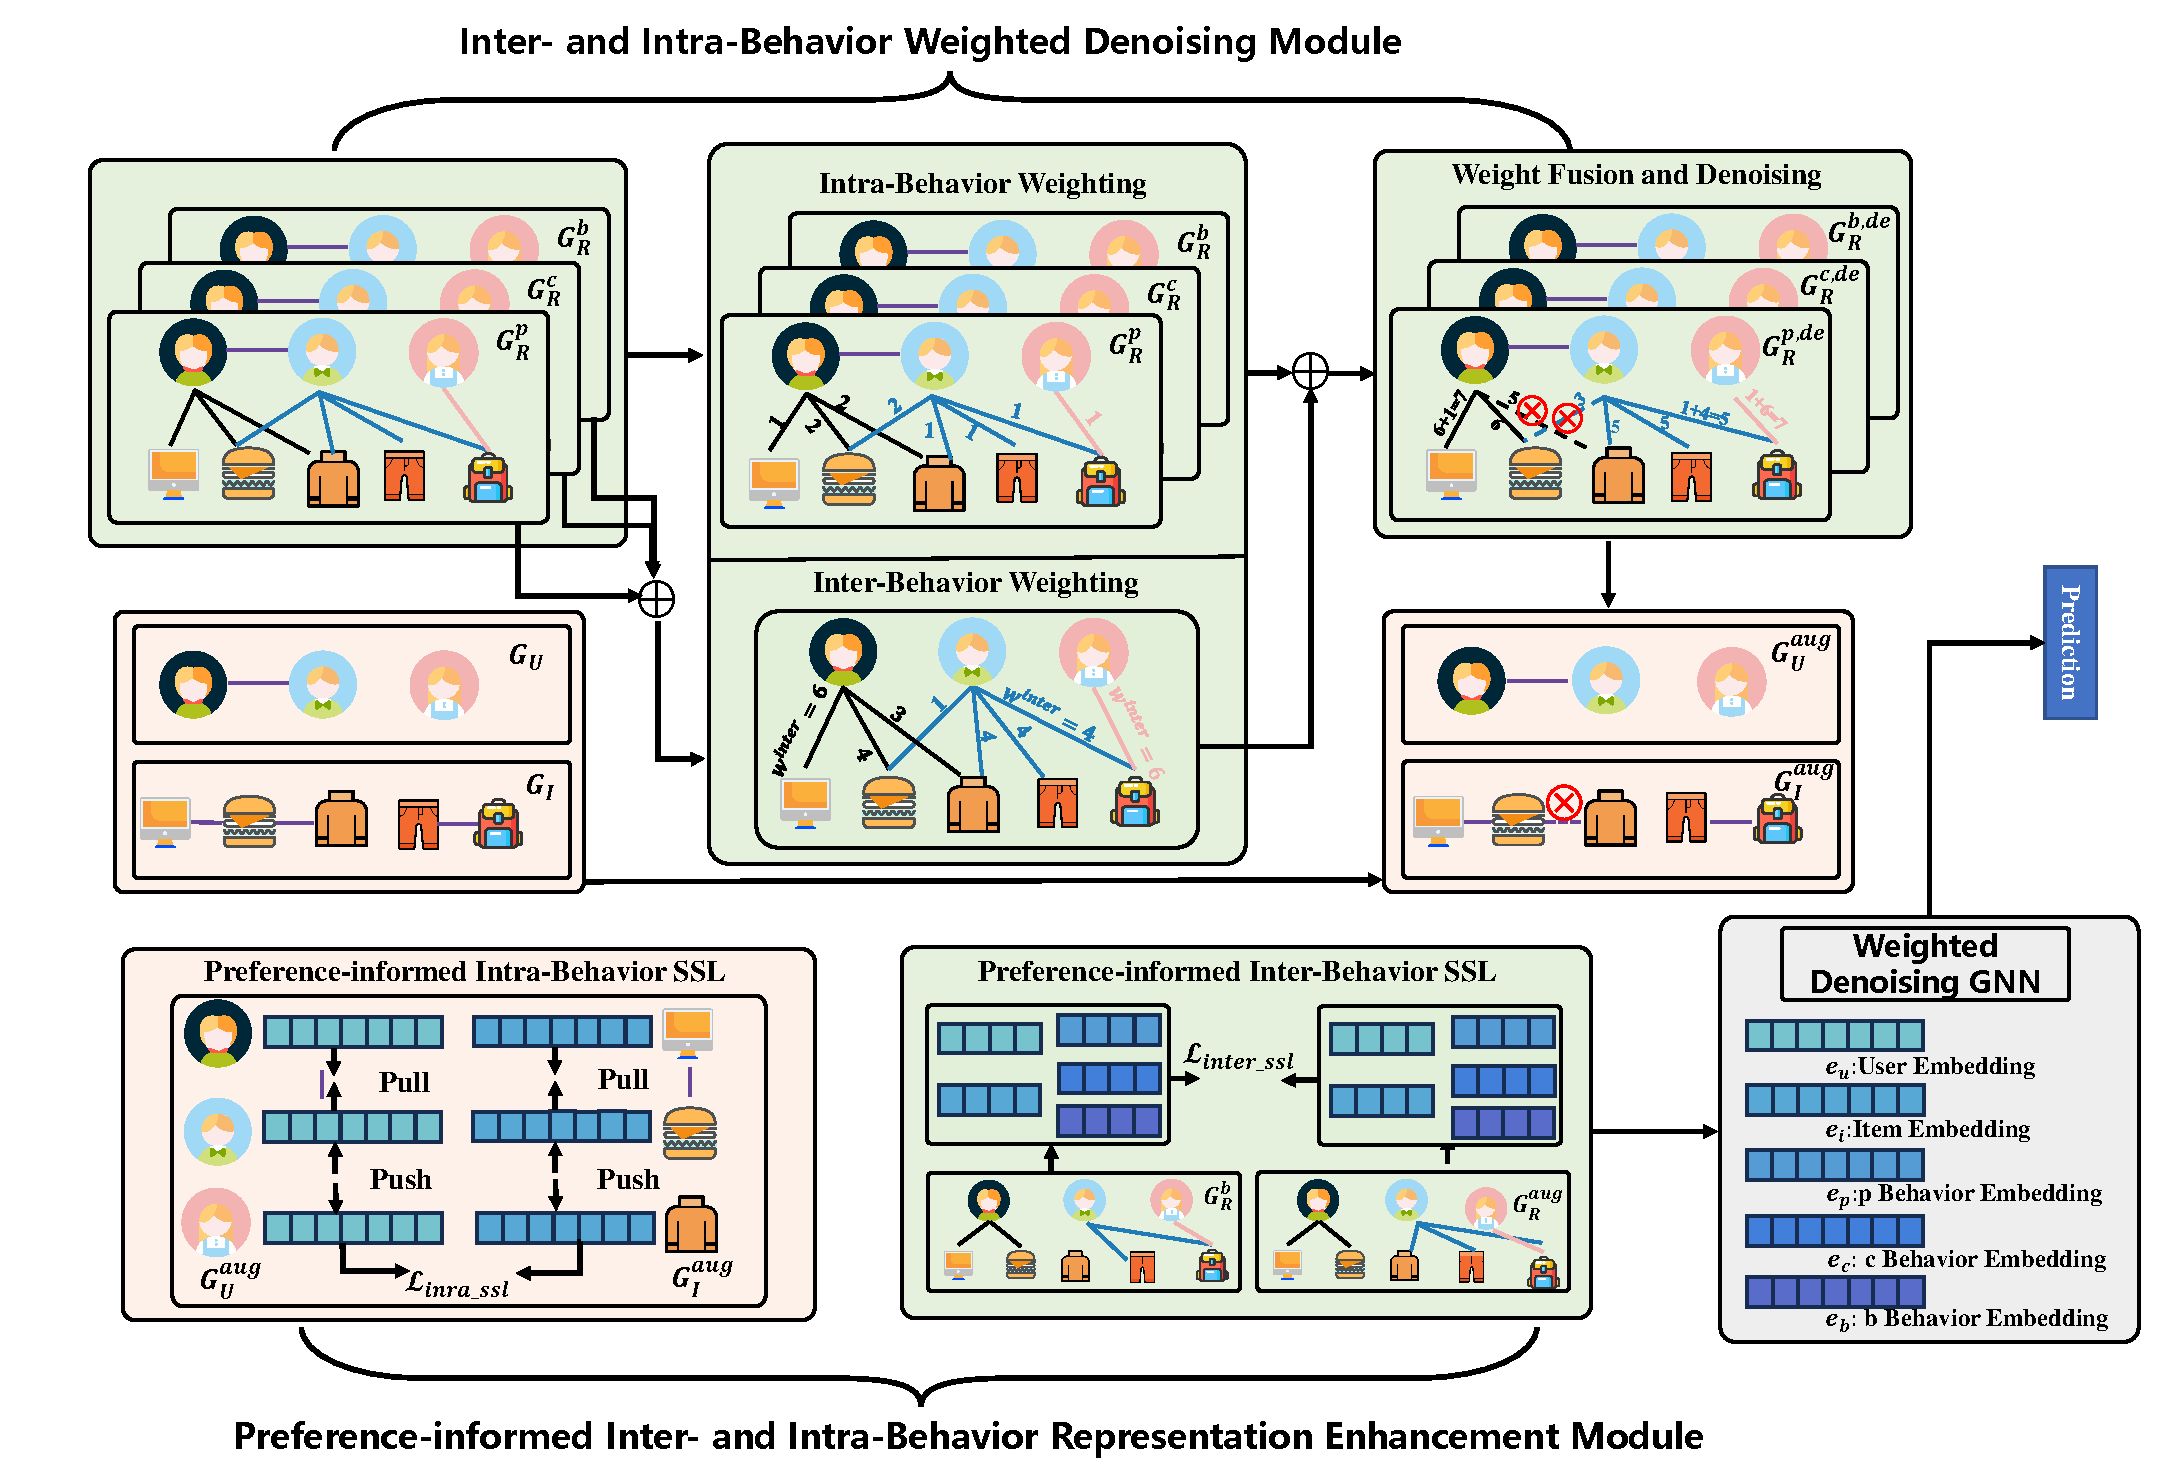
\includegraphics[width = 1.0\textwidth]{figures/model.pdf}
\caption{NIPER整体框架示意图}
\label{fig:model}
\end{figure}

为有效解决多行为推荐算法中的噪声干扰问题，本文提出了\textbf{噪声感知与偏好提取的多行为推荐方法}（NIPER: Noise Identification and Preference Extraction in Multi-Behavior Recommender System）。图~\ref{fig:model} 展示了 NIPER 的整体结构，该模型主要由两个关键模块组成：\textbf{(i) 行为间与行为内加权去噪模块（Inter- and Intra-Behavior Weighted Denoising Module）}与\textbf{(ii) 偏好感知的表征增强模块（Preference-informed Representation Enhancement Module）}。

\begin{enumerate}
    \item \textbf{行为间与行为内加权去噪模块}旨在识别并减轻辅助行为中的噪声交互，通过跨行为与行为内加权机制提升多行为信号的可靠性。该模块包含三个子模块：\textbf{基于行为强度的行为间加权模块}、\textbf{基于共同交互的行为内加权模块}以及\textbf{去噪模块}。  
    其中，基于行为强度的行为间加权模块用于刻画不同行为类型在用户偏好表达中的固有强度差异。例如，在电商场景中，购买行为通常较加购行为更能体现真实兴趣，而加购行为的偏好强度又高于单纯的浏览行为。  
    基于共同交互的行为内加权模块则用于建模具有相似兴趣的用户之间的交互影响。若多个用户在某些物品上表现出一致的交互行为，则这些行为更可能反映其真实偏好，从而获得更高的权重。  
    通过上述两类加权机制的协同作用，可构建出带有权重的多行为交互图。随后，去噪模块根据权重分布剔除低置信度的辅助行为交互，从而生成经过降噪处理且保留关键信息的高质量多行为图，有效减弱噪声对推荐结果的负面影响。

    \item \textbf{偏好感知的表征增强模块}旨在从辅助行为中提取高置信度的真实偏好，以缓解目标行为数据的稀疏性。该模块包括两部分：\textbf{偏好感知的行为间对比学习}与\textbf{偏好感知的行为内对比学习}。  
    前者利用在去噪阶段保留的高权重辅助交互，对目标行为交互图进行增强与补充。通过对比增强前后目标行为的嵌入表示，挖掘用户在多行为数据中的潜在偏好，从而提升整体推荐性能。  
    后者依据用户与用户、物品与物品之间的相似交互偏好，对其嵌入进行区分与优化，强化具有相似兴趣实体间的表示一致性，进一步提升模型的表达能力与泛化性。
\end{enumerate}

\section{行为间与行为内加权去噪模块}

在多行为推荐系统中，传统方法通常将用户行为划分为辅助行为与目标行为 \cite{chen2021GHCF, gu2022S-MBRec, zhang2023DPT, xu2023MBSSL, jin2020MBGCN, xia2021MB-GMN}。然而，这种二元划分忽略了不同辅助行为在表达用户兴趣偏好方面的重要性差异。例如，\textit{加入购物车}行为相较于\textit{浏览页面}更能反映用户的潜在购买意图。若不加区分地处理所有辅助行为，可能导致关键行为信号被削弱，从而降低推荐精度。

为定量刻画不同行为类型在购买转化中的作用，本文将点击与加购行为的影响建模为一个\textbf{因果推断问题} \cite{yao2021survey}，并采用\textbf{潜在结果框架}（Potential Outcomes Framework）\cite{huang2012assessing, 1025304585.nh}进行建模。  
对于每个用户 $i$，设 $T \in \{1, 2\}$ 表示行为类型，其中 $T=1$ 表示点击行为，$T=2$ 表示加购行为；$Y \in \{0, 1\}$ 表示用户是否完成购买；$X$ 表示用户的行为特征，包括点击次数、加购次数及总交互次数。

个体化处理效应（Individual Treatment Effect, ITE）定义为：
\begin{equation}
    \tau_i = \mathbb{E}[Y_i(2) - Y_i(1) \mid X_i],
\end{equation}
其中 $Y_i(t)$ 表示用户 $i$ 在行为类型 $T=t$ 下的潜在购买结果。由于实际数据中每个样本仅能观测到一个处理结果，因此需通过因果推断方法进行估计。

本文采用\textbf{因果森林模型（Causal Forest）}对 $\tau_i$ 进行估计。该模型是一种基于随机森林的非参数方法，能够在高维协变量空间中捕捉异质性处理效应。训练完成后，模型根据用户特征 $X_i$ 计算估计的处理效应：
\begin{equation}
    \tau_i = \hat{\mathbb{E}}[Y_i \mid T=2, X_i] - \hat{\mathbb{E}}[Y_i \mid T=1, X_i].
\end{equation}
若 $\tau_i > 0$，说明对用户 $i$ 而言，加购行为相较点击行为更能促进购买转化；反之则表示点击行为更具影响力。该效应可用于刻画不同行为的相对重要性。

为进一步量化各行为的强度，本文依据用户级处理效应 $\tau_i$ 构建行为权重。将其映射为点击与加购行为的响应权重如下：
\begin{equation}
    w_{\text{cart}, i} = \frac{\exp(\tau_i)}{\exp(\tau_i) + 1}, \quad
    w_{\text{click}, i} = 1 - w_{\text{cart}, i}.
\end{equation}
上述形式保证了权重的平滑性与归一性，能够有效反映用户在两种行为间的相对偏好强度。

基于用户级权重，定义加购行为的全局强度指标为：
\begin{equation}
    \rho^{\text{cart}} = \frac{1}{N} \sum_{i=1}^{N} w_{\text{cart}, i},
\end{equation}
相应地，点击行为的全局强度可表示为 $\rho^{\text{click}} = 1 - \rho^{\text{cart}}$。  
上述强度值用于衡量不同行为在全局范围内对购买转化的平均促进作用。作为最终目标行为，购买行为直接反映用户的真实转化，因此其强度设为常数：
\begin{equation}
    \rho^{\text{buy}} = 1.
\end{equation}

基于计算得到的各行为强度值，本文构建了全局加权的跨行为交互图 $\boldsymbol{G_{inter}}$，其邻接矩阵 $\boldsymbol{w^{inter}} \in \mathbb{R}^{|U| \times |I|}$ 定义为：
\begin{equation}
    w^{inter}_{ui} =  \sum_{k=1}^{K}\rho^{k} \cdot R^k_{ui}.
\end{equation}
该公式将多种行为的贡献进行加权融合，从而更全面地刻画用户的真实偏好与意图。如图~\ref{fig:w_inter} 所示，若用户 $u_1$ 在浏览、加购与购买三种行为中均与物品 $i_1$ 发生交互，则其全局权重为：
\begin{equation}
    w^{inter}_{u_{1}i_{1}} = w^{pv} \times 1 + w^{cart} \times 1 + w^{buy} \times 1 = 6.
\end{equation}
若用户 $u_1$ 仅在浏览与购买行为中与物品 $i_2$ 交互，则权重计算为：
\begin{equation}
    w^{inter}_{u_{1}i_{2}} = w^{pv} \times 1 + w^{cart} \times 0 + w^{buy} \times 1 = 4.
\end{equation}
通过上述建模过程，跨行为加权机制能够有效捕捉不同行为类型对用户偏好的贡献，为后续去噪与特征学习奠定基础。

\begin{figure}[h]
\centering
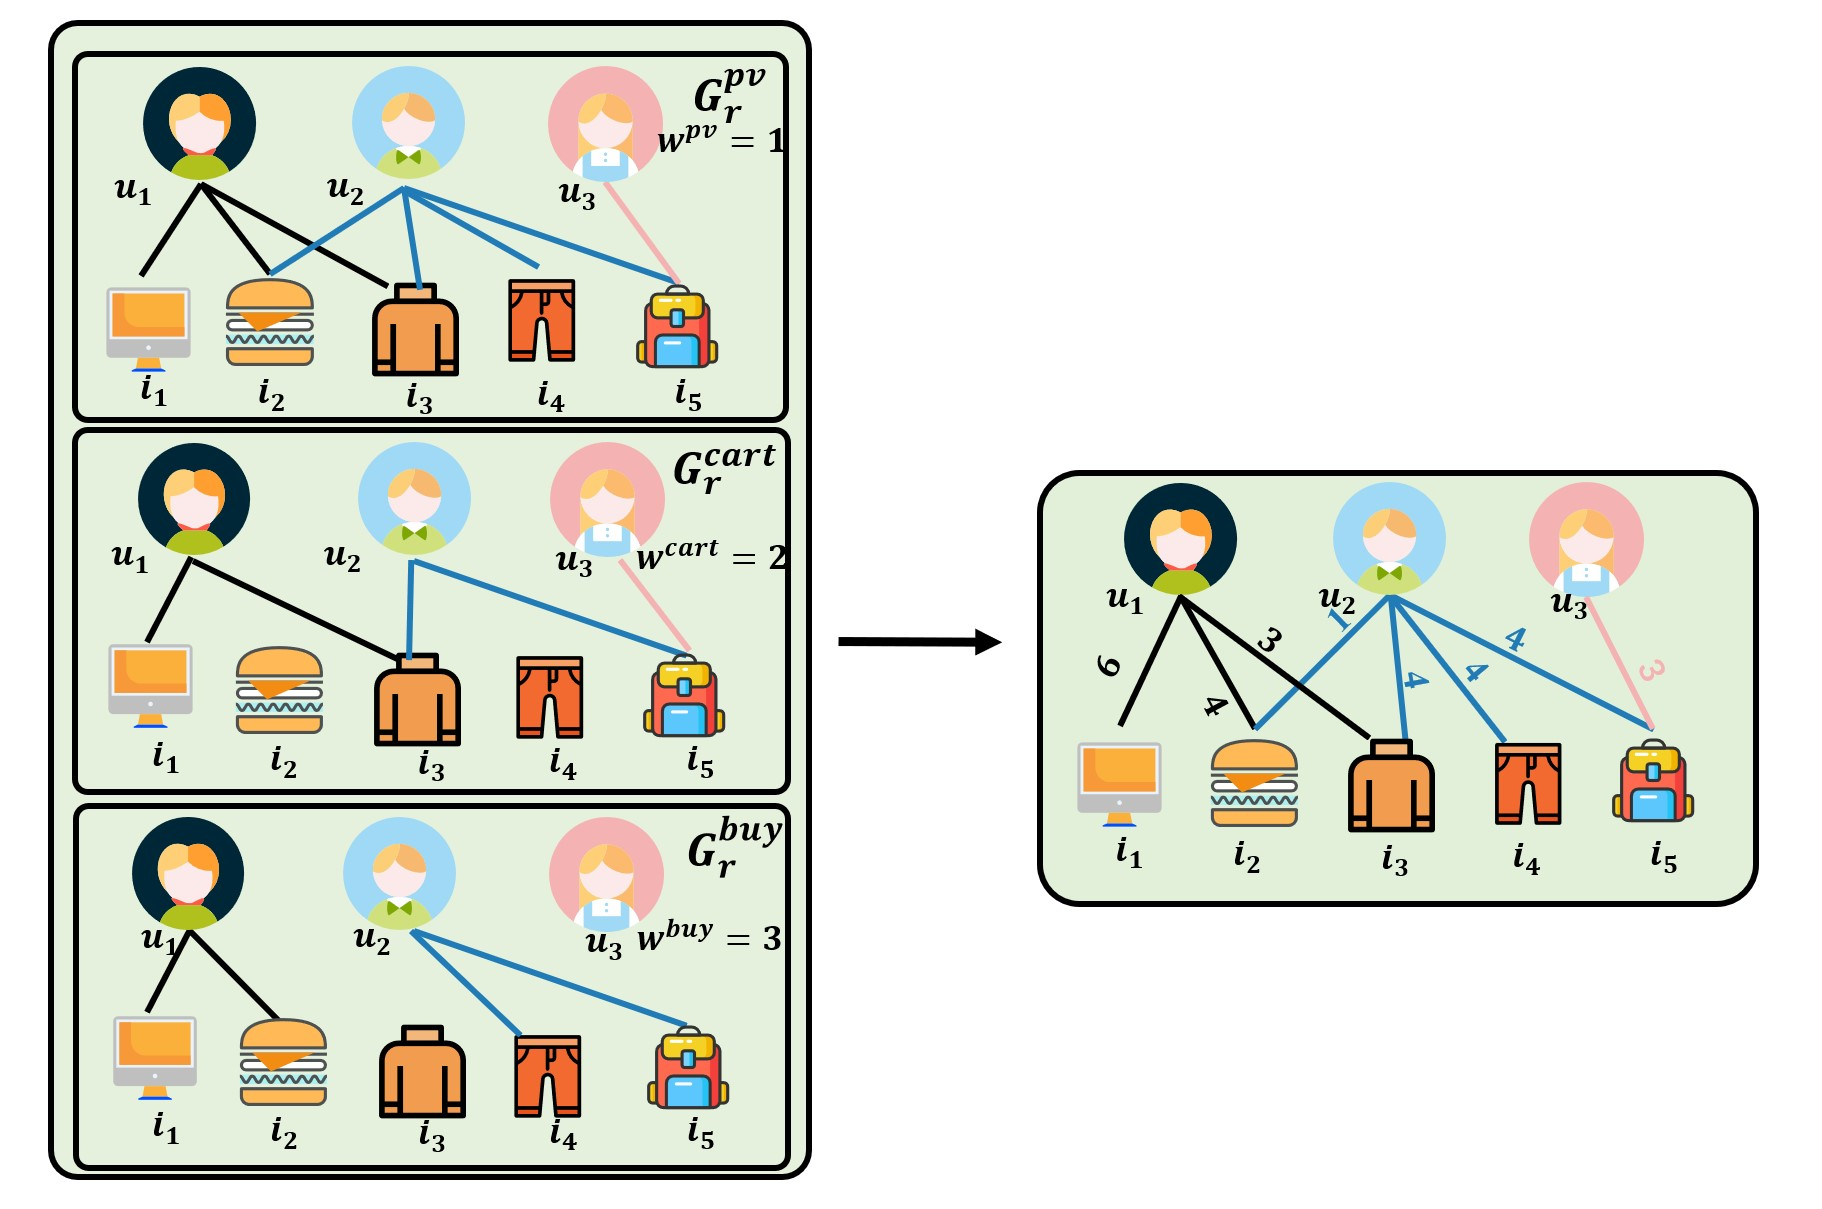
\includegraphics[width = 0.80\textwidth]{figures/w_inter.jpg}
\caption{一个生成带有权重的行为间全局交互图的例子}
\label{fig:w_inter}
\end{figure}

\textbf{基于共现交互的行为内加权：}
除了考虑不同行为类型在偏好表达中的强度差异外，用户在同一行为下的交互偏好同样蕴含着重要信息。这些偏好能够反映交互行为的相对重要性，并在相似用户之间体现出一定的一致性。基于此，本文引入\textbf{共现交互机制}，以量化具有相似兴趣的用户在同一行为下的共同交互强度。

具体而言，若相似用户在相同行为下频繁与同一物品交互，则该交互更可能代表真实偏好。为刻画这一关系，结合用户相似性交互图 $\boldsymbol{G_U}$ 与用户–物品交互图 $\boldsymbol{G_R}$，定义用户 $u$ 在行为 $k$ 下与物品 $i$ 的行为内权重如下：
\begin{equation}
    w^{\text{intra}, k}_{ui} = \Big( 1 + \sum_{v \in V_{u}} R^k_{vi} \Big) \cdot R^k_{ui},
\end{equation}
其中，$V_{u}$ 表示与用户 $u$ 相似的用户集合。该定义综合了用户相似性与共同交互频率，从而能够更全面地量化行为内交互的重要性。

为统一不同层次的权重信息，本文提出一种\textbf{行为内与行为间权重融合框架}。其中，行为内权重用于刻画单一行为下用户–物品交互的重要性，而跨行为权重用于建模不同行为类型间的关联性。两者的融合能够在全局层面上平衡行为差异与局部特征，从而更准确地反映用户的真实偏好。

在融合过程中，为避免权重尺度差异导致偏移，首先采用最小–最大归一化对行为内权重进行标准化。最终得到的融合权重矩阵 $\boldsymbol{w^{com, k}} \in \mathbb{R}^{|\mathcal{U}| \times |\mathcal{I}|}$ 定义如下：
\begin{equation}
    w^{\text{com}, k}_{ui} = \alpha w^{\text{intra}, k}_{ui} + (1 - \alpha) w^{\text{inter}}_{ui},
    \label{eq:w-com}
\end{equation}
其中，$k$ 表示行为类型，$\alpha$ 为平衡系数，用于控制行为内权重与跨行为权重的贡献比例。

\textbf{权重引导的去噪模块：}
该模块旨在进一步去除辅助行为中噪声交互的影响。具体而言，仅对辅助行为中权重较低的交互进行过滤，而目标行为保持不变。设每个辅助行为的融合权重为 $w^{\text{com},k}_{ui}$，并根据超参数 $\beta_{\text{low}}$ 及行为强度 $\rho^k$ 自适应确定去噪阈值，则去噪后的交互矩阵定义为：
\begin{equation}
    R_{ui}^{\text{de},k} = w_{ui}^{\text{com}, k} \cdot 
    \mathbb{I}\left(\frac{w_{ui}^{\text{com}, k}}{\max(\mathbf{w^{\text{com}, k}})} < 
    \frac{\beta_{\text{low}}}{\rho^k}\right),
\end{equation}
其中，$\mathbb{I}(\cdot)$ 表示指示函数。该机制确保仅去除低权重的辅助行为交互，而目标行为矩阵 $\boldsymbol{R^{\text{de},K}}$ 保持不变，直接令 $\boldsymbol{R^{\text{de},K}} = \boldsymbol{w^{\text{com},K}}$。  
最终，对于每个辅助行为 $k$，去噪后的矩阵 $\boldsymbol{R^{\text{de},k}}$ 保留了高置信度的交互信息，并作为相应去噪多行为图的邻接矩阵。该过程使得用户–物品交互关系能够被更准确、鲁棒地建模。

在得到多行为去噪加权交互矩阵 $\boldsymbol{R^{de,k}}$ 后，采用带有消息传递机制的图神经网络（GNN）对用户和物品进行表示学习。具体而言，本文以 GHCF（Graph-based Hybrid Collaborative Filtering）\cite{chen2021GHCF} 作为主干网络。GHCF 是一种针对多行为推荐任务设计的图神经网络结构，能够联合嵌入图中节点（用户与物品）及多种行为关系的表示，并显式捕获跨行为的高阶协同信号。

与原始 GHCF 在节点表示学习中对同一行为下的邻居进行等权聚合不同，本文在消息传播过程中引入了基于去噪权重的加权机制，使模型能够根据交互置信度动态调整邻居节点的重要性。其消息传播公式定义如下：
\begin{equation}
    \mathbf{e}^{(l+1)}_{u,k} = \text{LeakyReLU}\left(
    \mathbf{W}^{(l)} \cdot 
    \text{mean}\left\{
    \mathbf{e}^{(l)}_{i,k} \odot \mathbf{e}^{(l)}_{k} : i \in N_{u,k}
    \right\}
    \right),
\end{equation}
其中，$\mathbf{e}^{(l+1)}_{u,k}$ 表示在第 $(l+1)$ 层传播后，用户 $u$ 在行为类型 $k$ 下的嵌入表示；$N_{u,k}$ 为用户 $u$ 在行为 $k$ 下的邻居物品集合；$\mathbf{W}^{(l)}$ 为第 $l$ 层的特征变换矩阵；$\odot$ 表示逐元素乘积操作；$\mathbf{e}^{(l)}_{k}$ 为第 $l$ 层行为类型 $k$ 的全局嵌入向量，用于调节不同行为语义间的表示差异。

行为类型嵌入 $\mathbf{e}^{(l)}_{k}$ 在各层间通过以下线性变换进行更新：
\begin{equation}
    \mathbf{e}^{(l+1)}_{k} = \mathbf{W}^{(l)}_{b} \mathbf{e}^{(l)}_{k},
\end{equation}
其中，$\mathbf{W}^{(l)}_{b}$ 为层特定的行为类型转换矩阵，用于捕获多行为之间的语义迁移关系。

经过多层消息传播后，模型最终得到用户嵌入 $\mathbf{E_{u}}$、物品嵌入 $\mathbf{E_{i}}$ 以及行为类型嵌入 $\mathbf{E_{k}}$（其中 $k \in \mathcal{B}$），为后续的偏好建模与预测提供高质量的表示基础。

\section{偏好感知的表征增强模块}
\textbf{偏好感知的行为间对比学习：}
为缓解目标行为中的数据稀疏问题，本文利用辅助行为中高权重的交互信息对目标行为进行增强，从而构建更具代表性的交互视图。该方法通过将辅助行为中反映用户真实偏好的交互迁移至目标行为的表示空间，有效提升了目标行为的表达能力与鲁棒性。

具体而言，首先将所有辅助行为的去噪加权交互矩阵进行融合，定义如下：
\begin{equation}
    \boldsymbol{R^{all}} = \sum_{k=1}^{K-1} \boldsymbol{R^{de,k}},
\end{equation}
其中，$\boldsymbol{R^{all}}$ 表示合并后的多行为交互矩阵。为控制注入目标行为的辅助数据规模，引入阈值超参数 $\beta_{\text{high}}$，从辅助行为中筛选出高置信度的交互样本，得到高权重交互矩阵：
\begin{equation}
    R_{ui}^{\text{high}} = R_{ui}^{\text{all}} \cdot 
    \mathbb{I}\!\left(
    \frac{R_{ui}^{\text{all}}}{\max(\mathbf{R^{all}})} 
    \geq 1 - \beta_{\text{high}}
    \right),
    \label{eq:w-all}
\end{equation}
其中，$\mathbb{I}(\cdot)$ 为指示函数。将高权重矩阵 $\boldsymbol{R^{high}}$ 与目标行为的去噪矩阵 $\boldsymbol{R^{de,K}}$ 合并后，得到增强后的目标行为视图：
\begin{equation}
    \boldsymbol{R^{aug}} = \boldsymbol{R^{high}} + \boldsymbol{R^{de,K}}.
\end{equation}
该矩阵 $\boldsymbol{R^{aug}}$ 作为增强图 $\boldsymbol{G_{R}^{aug}}$ 的邻接矩阵，用于刻画用户与物品之间的强化交互关系。

上述过程生成了目标行为的两个视图：原始视图与增强视图。分别对两者进行编码后，得到节点表示 $\boldsymbol{e}^{\text{ori}}_{u}$ 与 $\boldsymbol{e}^{\text{aug}}_{u}$。节点级的正样本对定义为：
\[
\left\{
(\boldsymbol{e}^{\text{ori}}_{u}, \boldsymbol{e}^{\text{aug}}_{u}) \mid u \in \mathcal{U}
\right\},
\]
而负样本对为：
\[
\left\{
(\boldsymbol{e}^{\text{ori}}_{u}, \boldsymbol{e}^{\text{aug}}_{v}) \mid u, v \in \mathcal{U}, u \ne v
\right\}.
\]
在用户侧，优化目标采用 InfoNCE 损失定义如下：
\begin{equation}
    \mathcal{L}_{\text{inter,user}} =
    \sum_{u \in \mathcal{U}}
    -\log
    \left(
    \frac{
    \exp\left(\phi(\boldsymbol{e}^{\text{ori}}_{u}, \boldsymbol{e}^{\text{aug}}_{u}) / \tau\right)
    }{
    \sum_{v \in \mathcal{U}}
    \exp\left(\phi(\boldsymbol{e}^{\text{ori}}_{u}, \boldsymbol{e}^{\text{aug}}_{v}) / \tau\right)
    }
    \right),
\end{equation}
其中，$\tau$ 为温度系数，$\phi(\cdot)$ 表示内积运算。物品侧的损失函数可按相同方式计算，最终跨行为对比学习的总体损失为：
\begin{equation}
    \mathcal{L}_{\text{inter}} = 
    \mathcal{L}_{\text{inter,user}} + 
    \mathcal{L}_{\text{inter,item}}.
\end{equation}

\textbf{偏好感知的行为内对比学习：}
在多行为推荐中，具有相似交互模式的用户往往在偏好特征上表现出一致性，因此其嵌入表示也应保持高度相似。为此，本文引入了行为内对比学习机制，通过最大化相似用户嵌入之间的一致性，强化同偏好用户在表示空间中的聚合性，从而提升模型对用户真实偏好的刻画能力。

具体而言，基于增强后的交互矩阵 $\boldsymbol{R^{aug}}$，重新定义用户真实偏好相似性图 $\boldsymbol{G^{aug}_{U}}$ 与物品真实偏好相似性图 $\boldsymbol{G^{aug}_{I}}$。若用户 $u$ 与 $v$（或物品 $i$ 与 $j$）在 $\boldsymbol{R^{aug}}$ 中存在相同交互，则在用户图 $\boldsymbol{G^{aug}_{U}}$ 中建立 $u$ 与 $v$ 的连接，在物品图 $\boldsymbol{G^{aug}_{I}}$ 中建立 $i$ 与 $j$ 的连接。由此可以刻画用户（或物品）间的交互一致性关系。

基于上述图结构，将具有相似交互模式的用户视为正样本对 $(u, u^+)$，行为差异较大的用户视为负样本对 $(u, u^-)$。通过最大化正样本对之间的嵌入一致性并最小化负样本对之间的相似度，实现对用户嵌入空间的对比优化。设 $\boldsymbol{e}_u$ 表示用户 $u$ 的嵌入向量，行为内对比学习的目标函数定义如下：
\begin{equation}
    \mathcal{L}_{\text{intra,user}} = 
    \sum_{u \in \mathcal{U}} 
    -\log
    \left(
    \frac{
    \exp\left(\phi(\boldsymbol{e}_{u}, \boldsymbol{e}_{u^{+}}) / \tau\right)
    }{
    \sum_{u^{-} \in \mathcal{U}} 
    \exp\left(\phi(\boldsymbol{e}_{u}, \boldsymbol{e}_{u^{-}}) / \tau\right)
    }
    \right),
\end{equation}
其中，$u^{+}$ 表示与用户 $u$ 在图 $\boldsymbol{G^{aug}_U}$ 中相连的节点，$u^{-}$ 表示未与 $u$ 相连的节点；$\tau$ 为温度超参数，$\phi(\cdot)$ 表示内积相似度函数。物品侧的损失函数定义方式与用户侧相同，行为内对比学习的总目标为：
\begin{equation}
    \mathcal{L}_{\text{intra}} = 
    \mathcal{L}_{\text{intra,user}} + 
    \mathcal{L}_{\text{intra,item}}.
\end{equation}

\section{模型训练}
为实现稳定高效的模型训练，本文采用一种非采样推荐目标函数 \cite{chen2020EHCF}，其在准确性与效率上均优于传统的贝叶斯个性化排序（Bayesian Personalized Ranking, BPR）损失。对于给定的用户批次 $B$ 和物品集合 $\mathcal{I}$，在行为 $k$ 下的非采样推荐损失定义为：
\begin{equation}
    \mathcal{L}_{\text{rec}}^k =
    \sum_{u \in B} 
    \sum_{i \in I_u^{k+}} 
    \left[
    \left(c_i^{k+} - c_i^{k-}\right)
    \left(\hat{x}_{u,i}^k\right)^2 
    - 2c_i^{k+}\hat{x}_{u,i}^k
    \right],
\end{equation}
其中，$\hat{x}_{u,i}^k$ 表示用户 $u$ 在行为 $k$ 下对物品 $i$ 的预测交互概率；$I_u^{k+}$ 表示用户 $u$ 在行为 $k$ 下已发生交互的物品集合；$c_i^{k+}$ 和 $c_i^{k-}$ 为超参数，用于控制正负样本权重。

整体推荐任务的优化目标为各行为损失的加权和，其中 $\lambda_k$ 为各行为的平衡系数：
\begin{equation}
    \mathcal{L}_{\text{rec}} = 
    \sum_{k=1}^{K} 
    \lambda_k \mathcal{L}_{\text{rec}}^k.
\end{equation}

此外，本文在训练中引入自监督对比学习损失，以进一步提升嵌入表示的判别性与鲁棒性。最终的联合优化目标定义为：
\begin{equation}
    \mathcal{L} = 
    \mathcal{L}_{\text{rec}} + 
    \mu (\mathcal{L}_{\text{inter}} + \mathcal{L}_{\text{intra}}),
\end{equation}
其中，$\mu$ 为控制自监督学习强度的超参数。

训练完成后，目标行为下用户 $u$ 对未交互物品 $v$ 的交互概率计算如下：
\begin{equation}
    \hat{y}^{(k)}_{uv} = 
    \boldsymbol{e}_u^\top 
    \cdot 
    \text{diag}(\boldsymbol{e}_K) 
    \cdot 
    \boldsymbol{e}_v,
\end{equation}
其中，$\boldsymbol{e}_u$ 与 $\boldsymbol{e}_v$ 分别表示用户与物品的嵌入，$K$ 表示目标行为类型，$\text{diag}(\boldsymbol{e}_K)$ 为由目标行为嵌入构成的对角矩阵。

\section{实验与讨论}

\subsection{评价指标}
为了全面评估各模型在 Top-$K$ 推荐任务下的性能，本文选取了两个常用指标：召回率（Recall）和归一化折损累计增益（Normalized Discounted Cumulative Gain, NDCG）。对于测试集中的每个用户，模型首先对所有候选物品进行排序，并根据排序结果计算以下指标。

\begin{equation}
    \text{Recall@K} = 
    \frac{|R^{K}(u) \cap T(u)|}{|T(u)|},
\end{equation}

\begin{equation}
    \text{NDCG@K} = 
    \frac{1}{|U|} 
    \sum_{u \in U} 
    \frac{
        \sum_{k=1}^{K} 
        \frac{
            \mathbb{I}\left(R^K_k(u) \in T(u)\right)
        }{
            \log_2(k + 1)
        }
    }{
        \sum_{k=1}^{K} 
        \frac{1}{
            \log_2(k + 1)
        }
    },
\end{equation}
其中，$R^K(u)$ 表示模型为用户 $u$ 推荐的 Top-$K$ 个物品集合，$T(u)$ 表示测试集中用户 $u$ 实际交互（或点击）的物品集合，$R^K_k(u)$ 表示推荐列表中第 $k$ 个物品。$\mathbb{I}(\cdot)$ 为指示函数，当 $R^K_k(u) \in T(u)$ 时取 1，否则为 0。

Recall@K 反映模型能否成功推荐出用户真实感兴趣的物品，而 NDCG@K 则进一步关注这些物品在推荐列表中的排序位置。前者强调\textbf{推荐覆盖率}，后者衡量\textbf{推荐排序质量}。二者结合使用，可综合评估模型在多行为去噪推荐任务中的整体表现。


\begin{table}
\centering
\caption{数据集的统计信息}
\renewcommand{\arraystretch}{1.0}
\label{tab:dataset1}
\scalebox{0.9}{
\begin{tabular}{ccccccc}
\toprule
数据集 & \#User & \#Item & \#View & \#Cart & \#Favorite & \#Buy \\
\midrule
Beibei & 21,716 & 7,977 & 2,412,586 & 642,622 & -- & 282,860 \\
Taobao & 48,749 & 39,493 & 1,548,162 & 193,747 & -- & 211,022 \\
Tmall & 31,882 & 31,232 & 1,223,372 & 293,544 & 253,619 & 135,980 \\
\bottomrule
\end{tabular}
}
\end{table}

\subsection{数据集信息}
本研究选用了学术界广泛使用的三个多行为推荐数据集——Beibei、Taobao 和 Tmall，以评估所提出算法在不同场景下的有效性。  
这些数据集均包含用户与物品之间的多种交互行为（如浏览、收藏、加购与购买），能够充分反映用户在不同阶段的兴趣变化。  
所有数据集中均不包含显式反馈信息，仅记录用户的交互行为，因此非常适合用于基于隐式反馈的多行为去噪推荐研究。  
各数据集的详细统计信息见表~\ref{tab:dataset1}。

\subsection{实验设置}
实验在 PyTorch 框架下实现，优化器采用 Adam，学习率设为 0.001，批量大小为 256，嵌入维度为 64。  
为防止模型过拟合，在训练过程中设置嵌入丢弃率（embedding dropout rate）为 0.3，边丢弃率（edge dropout rate）为 0.1。  
非采样损失（non-sampling loss）中的负样本权重在 \{0.1, 0.01\} 中选择；对比学习的温度系数 $\tau$ 从 \{0.2, 0.4\} 中选取。  

\subsection{总体实验效果}
为验证所提出模型的有效性，本文选取了三类具有代表性的当前最先进推荐模型作为对比基线：

\begin{enumerate}
    \item \textbf{单行为推荐模型（Single-Behavior Recommendation Models）：}  
    此类模型仅利用目标行为进行训练，包括 NGCF~\cite{wang2019NGCF} 与 LightGCN~\cite{he2020lightgcn}。  
    此外，为评估将多种行为直接整合为单一行为的影响，构建了融合所有行为数据的单行为版本，分别记为 NGCF$_{\text{all}}$ 与 LightGCN$_{\text{all}}$。

    \item \textbf{去噪推荐模型（Denoising Recommendation Models）：}  
    包括面向单行为推荐的去噪方法 GraphDA~\cite{fan2023graphDA}，以及面向多行为推荐的去噪方法 DPT~\cite{zhang2023DPT}。

    \item \textbf{多行为推荐模型（Multi-Behavior Recommendation Models）：}  
    包括 S-MBRec~\cite{gu2022S-MBRec}、GHCF~\cite{chen2021GHCF}、MBSSL~\cite{xu2023MBSSL} 与 POGCN~\cite{zhang2024POGCN}。
\end{enumerate}

表~\ref{table:Comparison} 展示了 NIPER 与各类基线模型的实验结果，其中最佳与次优结果分别以加粗和下划线标注。  
综合结果表明，所提出方法在多项指标上均显著优于现有方法，具体分析如下：

\begin{enumerate}
    \item \textbf{NIPER 模型整体性能最优。}  
    NIPER 在 Recall 与 NDCG 等主要指标上均超越所有基线模型。  
    这一性能提升主要源于两点：  
    （1）跨行为与行为内加权去噪机制有效识别并削弱了辅助行为中的噪声干扰；  
    （2）偏好感知的表示增强模块在跨行为与行为内层面提升了嵌入的表达能力，使辅助行为中蕴含的真实偏好得以有效迁移至目标行为表示中。

    \item \textbf{多行为建模显著优于单行为建模。}  
    多行为推荐模型在三种数据集上均表现出优于单行为模型的效果，说明充分建模行为间关系能够更准确地反映用户的潜在偏好。  
    同时，将所有行为简单合并为单一行为（NGCF$_{\text{all}}$、LightGCN$_{\text{all}}$）虽略有提升，但仍显著落后于多行为建模方法。

    \item \textbf{辅助行为包含有价值偏好信息但同时存在噪声。}  
    在 Beibei 与 Taobao 数据集中，将辅助行为纳入建模能提升推荐性能，说明辅助行为中确实包含真实偏好信号。  
    然而在 Tmall 数据集中，该策略反而导致性能下降，表明该数据集的辅助行为中噪声比例更高，直接合并行为可能放大噪声影响。

    \item \textbf{NIPER 在去噪性能方面优于现有方法。}  
    与 GraphDA（单行为去噪）和 DPT（独立行为去噪）相比，NIPER 在考虑行为依赖关系的同时实现多行为联合去噪，  
    并结合自监督学习增强表示鲁棒性，从而在多行为场景下展现出更优的性能。
\end{enumerate}


\begin{table*}[htbp]
\renewcommand{\arraystretch}{1.0}
\caption{NIPER在三个数据集上的实验结果(Beibei, Taobao, Tmall)}
\centering
\begin{adjustbox}{width=1\textwidth}
\begin{tabular}{l|cccc|cccc|cccc}
\toprule
\multirow{2}{*}{Model} & \multicolumn{4}{c|}{Beibei} & \multicolumn{4}{c|}{Taobao} & \multicolumn{4}{c}{Tmall} \\
& R@5 & R@10 & N@5 & N@10 & R@5 & R@10 & N@5 & N@10 & R@5 & R@10 & N@5 & N@10\\
\midrule
NGCF \cite{wang2019NGCF} & 0.0185 & 0.0348 & 0.0108 & 0.0161 & 0.0203 & 0.0291 & 0.0141 & 0.0169 & 0.0219 & 0.0329 & 0.0146 & 0.0182  \\
NGCF${_{all}}$ \cite{wang2019NGCF}& 0.0316 & 0.0487 & 0.0194 & 0.0261 & 0.0254 & 0.0348 & 0.0193 & 0.0205 & 0.0024 & 0.0053 & 0.0021 & 0.0029\\
LightGCN \cite{he2020lightgcn} & 0.0230& 0.0419 & 0.0141 & 0.0202 & 0.0300 & 0.0412 & 0.0211 & 0.0247 & 0.0363 & 0.0524 & 0.0251 & 0.0303 \\
LightGCN${_{all}}$ \cite{he2020lightgcn}& 0.0349 & 0.0583 & 0.0222 & 0.0297 & 0.0377 & 0.0433 & 0.0284 & 0.0284 & 0.0036 & 0.0060 & 0.0023 & 0.0030\\
GraphDA \cite{fan2023graphDA}& 0.0384 & 0.0603 & 0.0253 & 0.0312 & 0.0318 & 0.0468 & 0.0214 & 0.0253 & 0.0153 & 0.0204 & 0.0098 & 0.0143\\
DPT \cite{zhang2023DPT}& 0.1009 & 0.1621 & 0.0545 & 0.0793 & 0.0484 & 0.1025  & 0.0375 & 0.0571 & 0.0573 & 0.0934 & 0.0353 & 0.0448\\
S-MBRec \cite{gu2022S-MBRec}& 0.0981 & 0.1697 & 0.0613 & 0.0872 & 0.0673 & 0.0814 & 0.0348 & 0.0446 & 0.0503	& 0.0639 & 0.0301 &	0.0397\\
GHCF \cite{chen2021GHCF}& \uline{0.1227} & \uline{0.1897} & \uline{0.0783} & \uline{0.1000} & 0.0534 & 0.0807 & 0.0361 & 0.0449 & 0.0462 & 0.0763 & 0.0287 & 0.0384\\
MBSSL \cite{xu2023MBSSL}& 0.1034 & 0.1734 & 0.0652 & 0.0899 & \uline{0.0688} & \uline{0.1022} & \uline{0.0465} & \uline{0.0567} & \uline{0.0507} & \uline{0.0838} & \uline{0.0313} & \uline{0.0419} \\
POGCN \cite{zhang2024POGCN}& 0.0854 & 0.1548 & 0.0621 & 0.0801 & 0.0519 & 0.0841 & 0.0351 & 0.0423 & 0.0458 & 0.0741 & 0.0214 & 0.0386   \\
NIPER & \textbf{0.1632} & \textbf{0.2372} & \textbf{0.1053} & \textbf{0.1292} & \textbf{0.0812} & \textbf{0.1084} & \textbf{0.0576} & \textbf{0.0664} & \textbf{0.0884} & \textbf{0.1216} & \textbf{0.0585} & \textbf{0.0693} \\ 
\bottomrule
\end{tabular}
\end{adjustbox}
\label{table:Comparison} 
\end{table*}

\subsection{消融实验}
为验证所提出模型中各个设计模块的有效性与必要性，本节进行了系统的消融实验。具体地，设计了以下六个模型变体：

\begin{enumerate}
    \item \textbf{w/o Inter-Weighting：} 移除跨行为加权机制，仅保留行为内权重进行去噪；
    \item \textbf{w/o Causal Inference：} 去除基于因果推断的行为强度估计，采用人工设定的固定值作为行为强度，其中 $\rho^{click}=1$，$\rho^{cart}=\rho^{collect}=2$，$\rho^{buy}=3$；
    \item \textbf{w/o Intra-Weighting：} 移除行为内加权机制，仅依赖跨行为权重进行去噪；
    \item \textbf{w/o Denoising：} 完全取消去噪模块，直接利用原始多行为交互图进行建模；
    \item \textbf{w/o SSL$_{\text{inter}}$：} 移除偏好增强模块中的跨行为自监督学习部分；
    \item \textbf{w/o SSL$_{\text{intra}}$：} 移除偏好增强模块中的行为内自监督学习部分。
\end{enumerate}

消融实验结果如表~\ref{table:ablation} 所示。由于篇幅限制，本文重点报告 Beibei 与 Taobao 数据集上的 Recall@5 结果，其他数据集上亦观察到相似趋势。结果分析如下：

\begin{enumerate}
    \item \textbf{加权机制的重要性。}  
    跨行为与行为内加权机制的结合能够有效整合多视角信息，对不同交互的重要性进行精细区分。  
    当任意一项加权机制被移除时（如 w/o Inter-Weighting 或 w/o Intra-Weighting），模型性能均出现明显下降，表明该双层加权策略对于识别噪声交互与保持有效信号均至关重要。

    \item \textbf{去噪模块的必要性。}  
    将完整模型与 w/o Denoising 变体对比可发现，去噪模块在显著提升模型精度方面起关键作用。  
    若直接使用未经筛选的原始交互，辅助行为中的噪声信号会误导用户偏好建模，导致推荐结果偏差。  
    因此，去噪阶段对于提升推荐系统的鲁棒性和准确性具有重要意义。

    \item \textbf{自监督学习增强的有效性。}  
    当移除自监督学习组件（w/o SSL$_{\text{inter}}$ 或 w/o SSL$_{\text{intra}}$）后，模型性能均明显下降。  
    这表明跨行为自监督学习（inter-SSL）通过高权重辅助行为增强目标行为表示，而行为内自监督学习（intra-SSL）有助于强化相似用户与物品之间的嵌入一致性。  
    二者协同作用显著提升了模型的表征能力与泛化性能。
\end{enumerate}


\begin{table}[h]
\renewcommand{\arraystretch}{0.8}
\centering
\caption{消融实验结果}
\scalebox{0.85}{
\begin{tabular}{lcccccccc}
\toprule
\multirow{2}{*}{DataSet} & \multicolumn{2}{c}{Beibei} & \multicolumn{2}{c}{Taobao} & \multicolumn{2}{c}{Tmall}\\
\cmidrule(r){2-3} \cmidrule(r){4-5} \cmidrule(r){6-7}
Metric & Recall@5 & NDCG@5 & Recall@5 & NDCG@5 & Recall@5 & NDCG@5\\
\midrule
w/o Inter-Weighting & 0.1243 & 0.0783 & 0.0704 & 0.0487 & 0.0611 & 0.0397 \\
w/o Casual Inference & 0.1325 & 0.0.0835 & 0.0806 & 0.0524 & 0.0691 & 0.0429 \\
w/o Intra-Weighting & 0.1232 & 0.0746 & 0.0720 & 0.0472 & 0.0601 & 0.0383\\
w/o Denoising & 0.1198 & 0.0758 & 0.0603 & 0.0406 & 0.0493 & 0.0318 \\
w/o SSL$_{\text{inter}}$ & 0.1154 & 0.0775 & 0.0618 & 0.0454 & 0.0576 & 0.0381\\
w/o SSL$_{\text{intra}}$ & 0.1163 & 0.0769 & 0.0605 & 0.0438 & 0.0549 & 0.0375 \\
NIPER & \textbf{0.1632} & \textbf{0.1053} & \textbf{0.0812} & \textbf{0.0576} & \textbf{0.0884} & \textbf{0.0585} \\
\bottomrule
\end{tabular}
}
\label{table:ablation} 
\end{table}

\subsection{参数实验}
为探究模型关键超参数对整体性能的影响，本文从噪声移除比例 $\beta_{low}$、目标行为增强比例 $\beta_{high}$ 以及行为权重平衡系数 $\alpha$ 三个方面进行了系统实验分析。  
图~\ref{fig:para} 展示了各参数变化对模型性能的影响趋势与差异。

\begin{enumerate}
    \item \textbf{去噪比例 $\beta_{low}$ 的影响：}  
    如图~\ref{fig:para}(a) 所示，不同数据集在最优去噪比例上的差异反映了其噪声水平的不同。  
    随着去噪比例的提高，模型性能呈现“先升后降”的趋势。  
    这一现象可归因于以下两点：（i）在较低的去噪比例下，适度去除噪声交互有助于减少无关信息的干扰；（ii）当比例过高时，部分有效交互被误删，导致模型无法充分学习用户的真实偏好，从而造成性能下降。

    \item \textbf{辅助行为增强比例 $\beta_{high}$ 的影响：}  
    增强比例 $\beta_{high}$ 控制辅助行为对目标行为的补充程度。  
    如图~\ref{fig:para}(b) 所示，随着 $\beta_{high}$ 的增大，模型性能初期逐步提升，但在超过最优值后出现下降。  
    这表明，适量引入辅助行为能够有效传递真实偏好信息，而过高的增强比例则会引入噪声或无效信号，反而削弱推荐效果。  
    因此，合理设定 $\beta_{high}$ 对于充分利用辅助行为、提升模型准确性至关重要。

    \item \textbf{平衡系数 $\alpha$ 的影响：}  
    参数 $\alpha$ 用于平衡行为间权重与行为内权重的重要性。  
    如图~\ref{fig:para}(c) 所示，当 $\alpha$ 取值过小或过大时，模型会分别过度依赖跨行为或行为内权重，从而造成性能下降。  
    虽然不同数据集的最优 $\alpha$ 值略有差异，但整体趋势表明，在两类权重间保持适当平衡能够使模型获得最佳表现。
\end{enumerate}

\begin{figure}[htbp]
    \centering
    % 第一行
    \begin{minipage}[t]{0.4\textwidth}
        \centering
        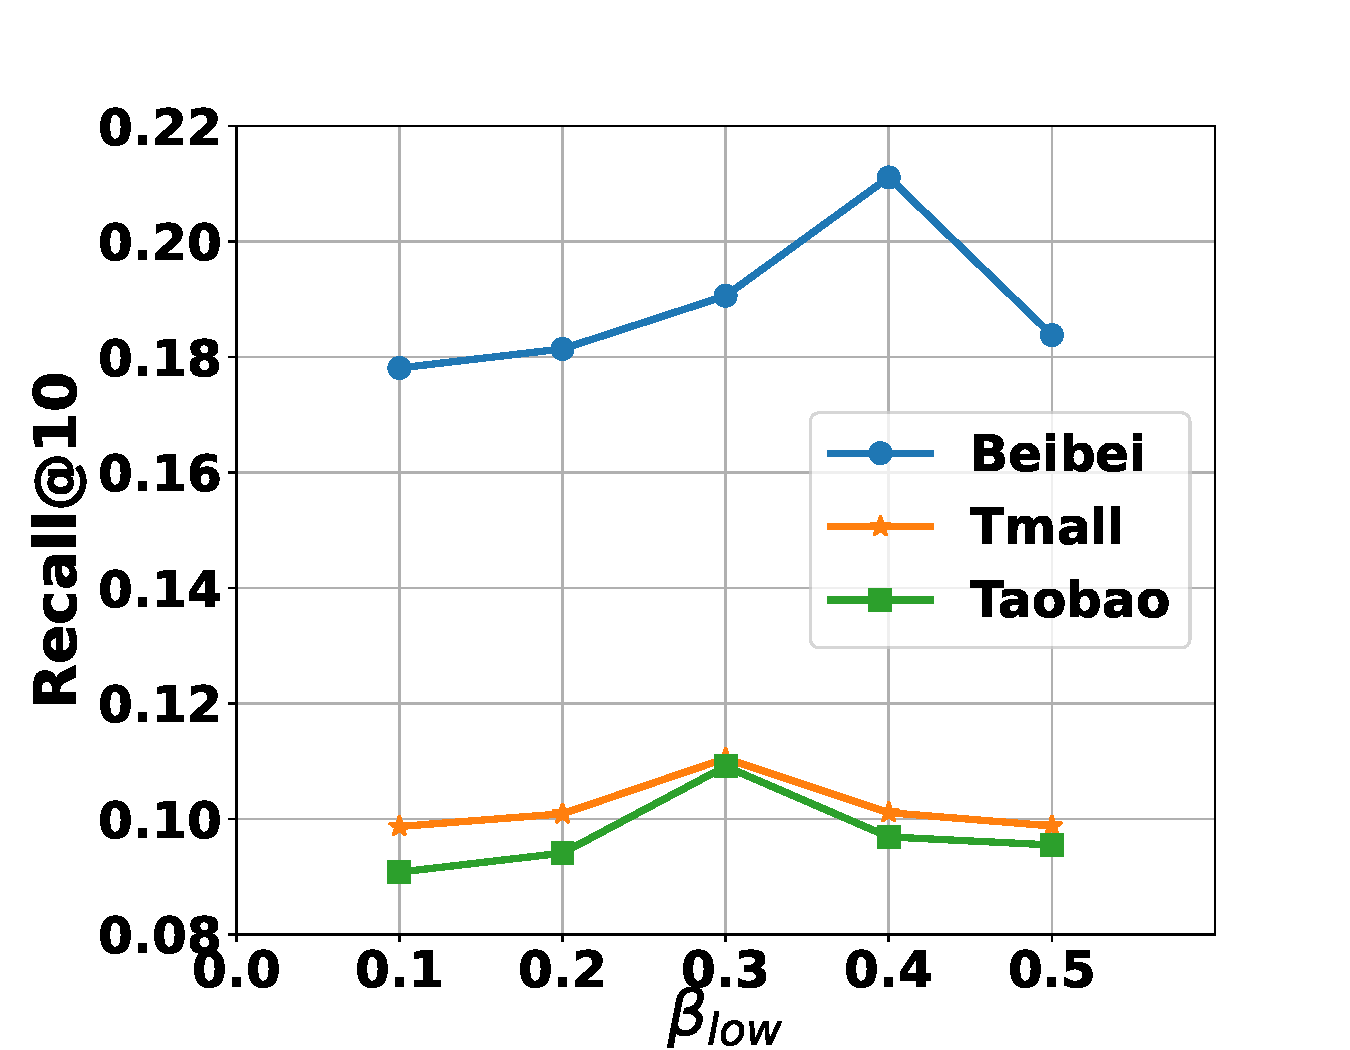
\includegraphics[width=\linewidth]{figures/low.pdf}
        \caption*{\small (a) 去噪比例 $\beta_{low}$}
    \end{minipage}
    \hspace{0.05\textwidth}
    \begin{minipage}[t]{0.4\textwidth}
        \centering
        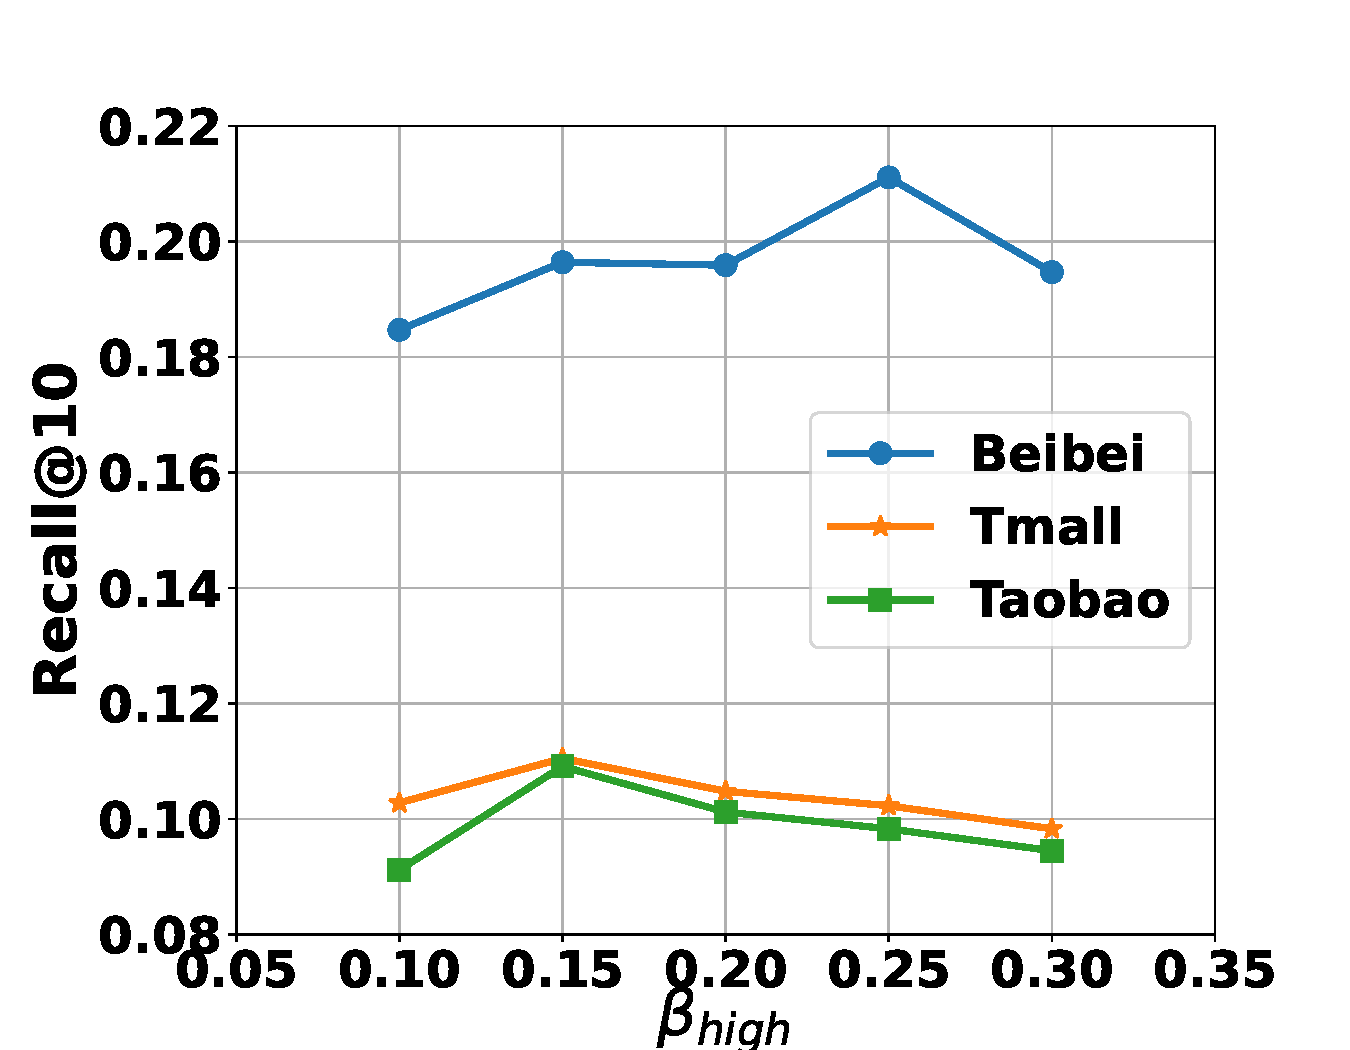
\includegraphics[width=\linewidth]{figures/high.pdf}
        \caption*{\small (b) 辅助行为增强比例 $\beta_{high}$}
    \end{minipage}
    % 第二行
    \begin{minipage}[t]{0.4\textwidth}
        \centering
        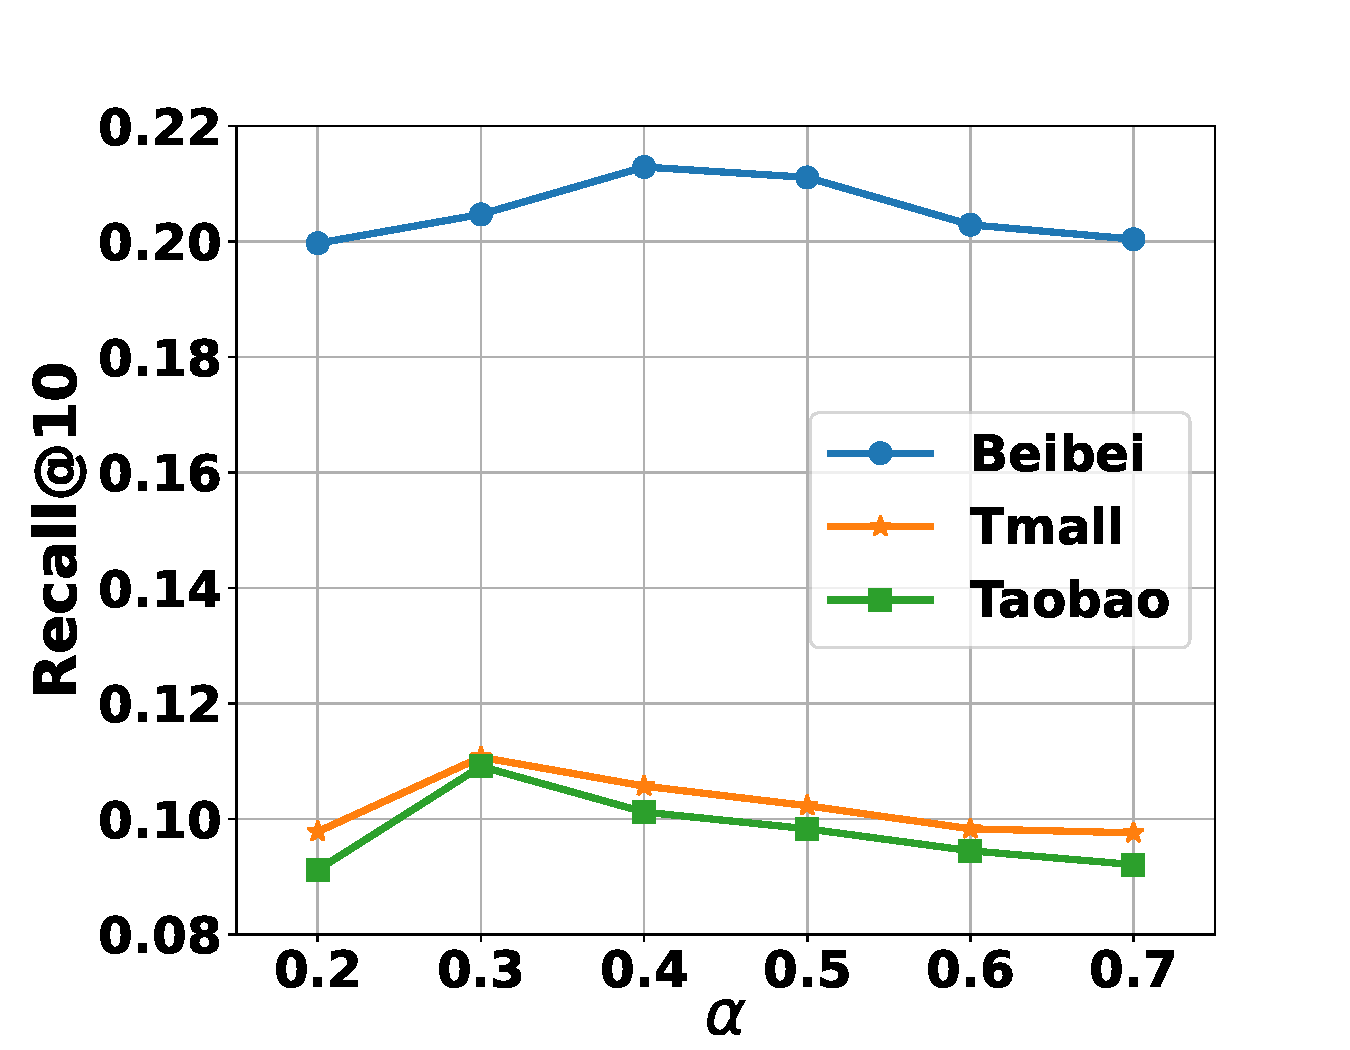
\includegraphics[width=\linewidth]{figures/alpha.pdf}
        \caption*{\small (c) 平衡系数 $\alpha$}
    \end{minipage}
    \hspace{0.05\textwidth}
    \caption{超参数实验}
    \label{fig:para}
\end{figure}

\subsection{案例研究}
\textbf{(1)去噪模块有效性分析}

为进一步验证所提出去噪模块的通用性与可迁移性，本节将 NIPER 的跨行为与行为内加权去噪模块集成至三种当前最先进的多行为推荐模型中——GHCF~\cite{chen2021GHCF}、MBSSL~\cite{xu2023MBSSL} 和 POGCN~\cite{zhang2024POGCN}，以评估其对不同框架的性能提升效果。  
实验采用 Recall@10 与 NDCG@10 两项指标，对集成去噪模块前后的性能差异进行对比分析，从而量化该模块在提升推荐精度方面的贡献。

\begin{figure}[h]
  \centering
  \begin{minipage}[t]{0.45\textwidth}
    \centering
    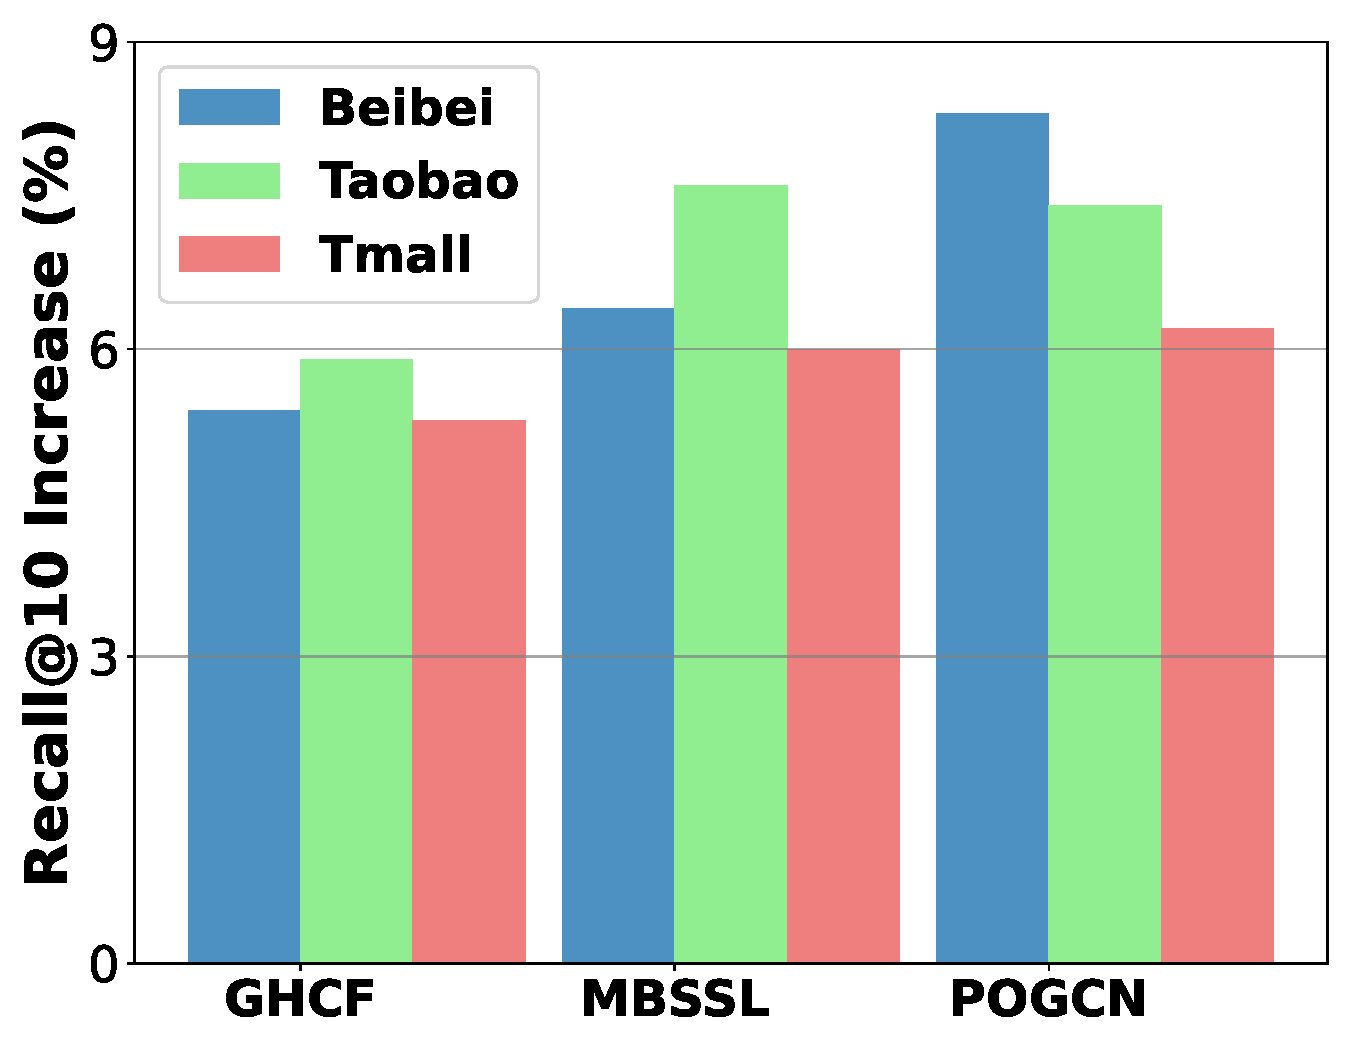
\includegraphics[width=0.9\linewidth]{figures/case_study1-Recall.pdf}
    \caption*{(a) Recall@10 提升效果}
    \label{fig:case1-Recall}
  \end{minipage}
  \hspace{0.05\textwidth}
  \begin{minipage}[t]{0.45\textwidth}
    \centering
    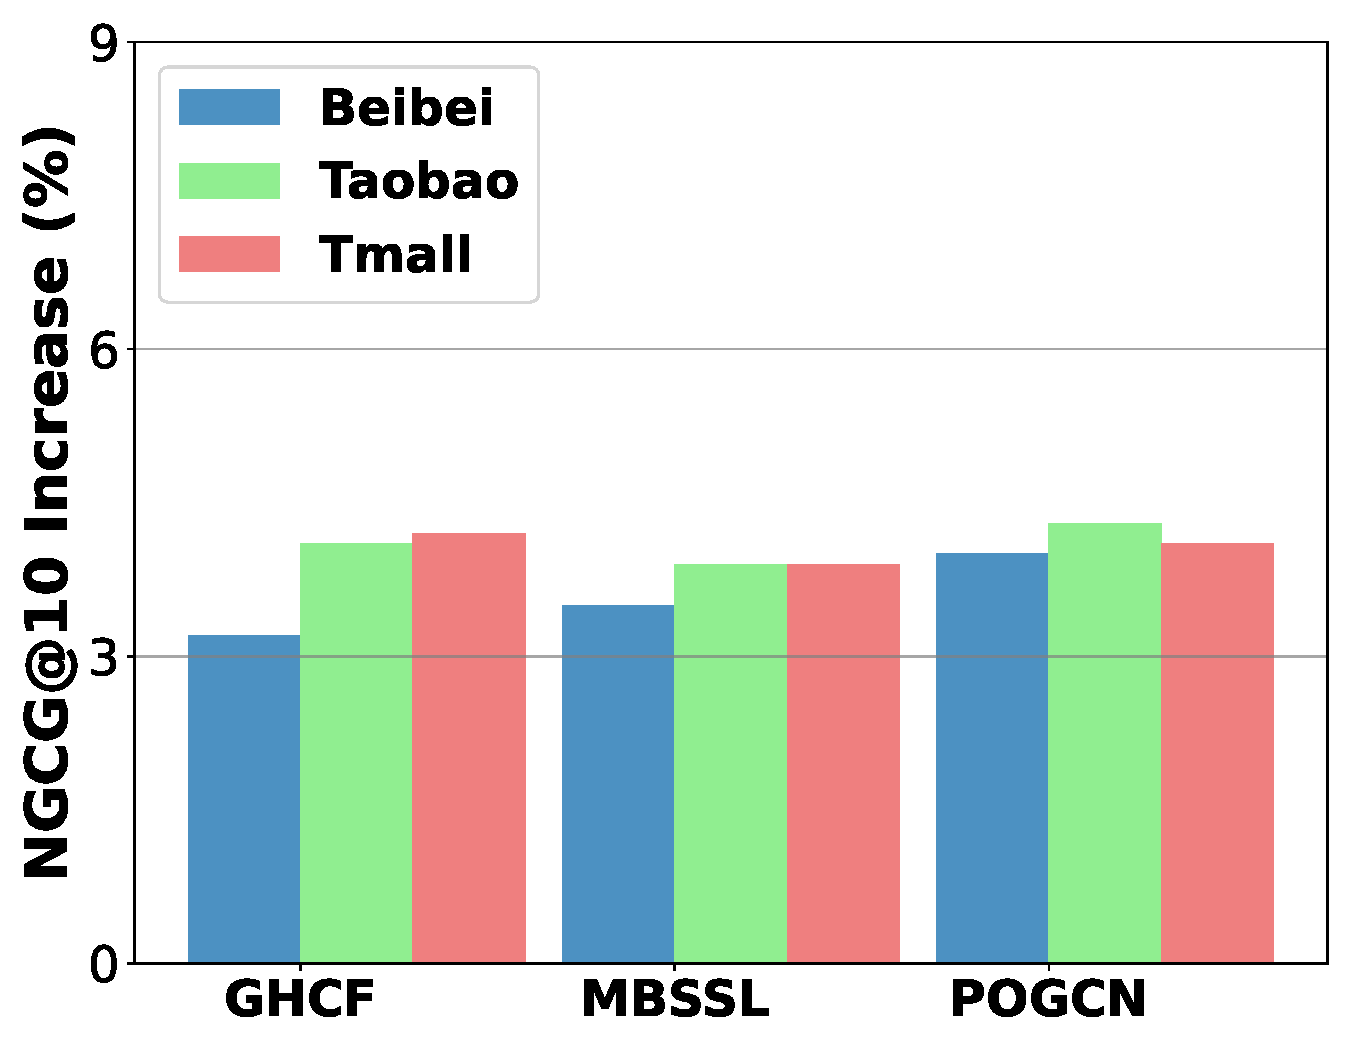
\includegraphics[width=0.9\linewidth]{figures/case_study1-NDCG.pdf}
    \caption*{(b) NDCG@10 提升效果}
    \label{fig:case1-NDCG}
  \end{minipage}
  \caption{在不同模型中集成 NIPER 去噪模块后的性能增益}
  \label{fig:case1}
\end{figure}

\begin{figure}[h]
  \centering
  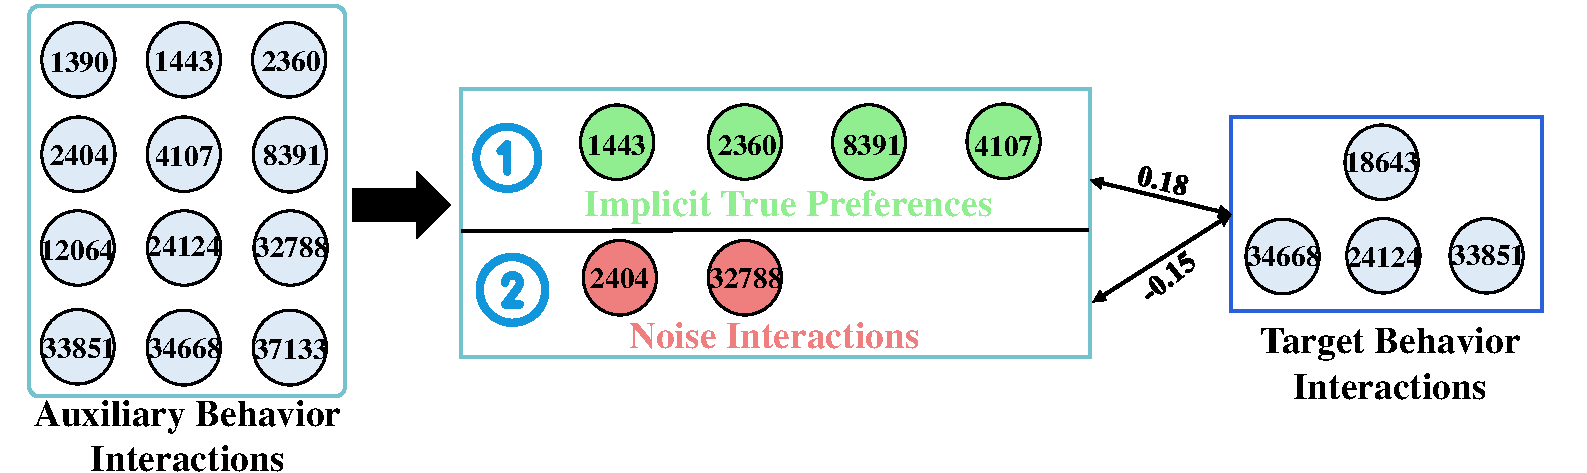
\includegraphics[width=1.0\linewidth]{figures/case_study2.pdf}
  \caption{辅助行为与目标行为相似性案例分析}
  \label{fig:case2}
\end{figure}

如图~\ref{fig:case1} 所示，在 Beibei、Taobao 和 Tmall 数据集上，三种基线模型在 Recall@10 与 NDCG@10 指标上均取得显著提升。  
该结果表明，NIPER 的去噪机制能够有效降低多行为交互中的噪声干扰，同时具备良好的通用性与可扩展性，可作为提升现有多行为推荐框架性能的独立模块。

\textbf{(2)去噪模块的局部效果分析}

为进一步验证 NIPER 在辅助行为分类中的有效性，本节从局部视角对其进行分析。我们选取 Taobao 数据集中的一位典型用户作为研究对象，该用户在辅助行为下与 12 个物品发生过交互。依据模型在最优参数设置下的权重分布，我们根据去噪阈值 $\beta_{low}$ 和增强阈值 $\beta_{high}$ 对该用户的辅助行为进行了分类。其中，权重低于 $\beta_{low}$ 的交互被视为噪声样本，而权重高于 $(1 - \beta_{high})$ 的交互则被认为更能反映用户的真实偏好。随后，我们计算辅助行为交互与用户实际购买物品之间的余弦相似度，以验证分类结果的合理性。

\textbf{分析：}如图~\ref{fig:case2} 所示，辅助行为中被识别为真实偏好的高权重交互，其与目标行为（购买行为）物品的相似度显著高于被识别为噪声的交互。这表明，NIPER 能够精准地区分噪声与真实偏好，在去除无效交互的同时，有效保留对用户真实兴趣具有代表性的交互信息，从而提升模型的整体推荐性能。

\section{本章小结}
本章提出了一种新颖的多行为推荐框架——NIPER（Noise Identification and Preference Extraction in Multi-Behavior Recommender System），用于解决多行为推荐系统中噪声交互与真实偏好提取的核心问题。与以往方法普遍将所有辅助行为数据直接融合到目标行为模型中不同，NIPER能够区分辅助行为中的噪声与真实偏好。
其中，跨行为与行为内加权去噪模块通过为多行为交互分配权重，有效削弱了噪声交互的影响，确保无关或偶然的行为被过滤；基于偏好的表征增强模块则利用自监督学习机制，从辅助行为中提取真实偏好信息，从而增强模型的表达能力。
在多个公开数据集上的广泛实验结果表明，NIPER 在推荐精度上显著优于现有最先进方法，验证了该框架在提升多行为推荐系统鲁棒性与准确性方面的有效性。